\documentclass[3p,times,procedia]{elsarticle}
\flushbottom

\usepackage{ecrc}
\usepackage[bookmarks=false]{hyperref}
\hypersetup{hidelinks}
\usepackage{amsmath,amssymb,amsfonts}
\usepackage{graphicx}
\usepackage{textcomp}
\usepackage{xcolor}
\usepackage{booktabs}
\usepackage{multirow}
\usepackage{float}
\usepackage{url}
\usepackage{acronym}
\usepackage[section]{placeins}

\volume{00}
\firstpage{1}
\journalname{Procedia Computer Science}
\runauth{A. Gargouri et al.}
\jid{procs}

\acrodef{hrc}[HRC]{Human-Robot Collaboration}
\acrodef{dt}[DT]{Digital Twin}
\acrodef{uda}[UDA]{Unsupervised Domain Adaptation}
\acrodef{gcn}[GCN]{Graph Convolutional Network}
\acrodef{ctrgcn}[CTR-GCN]{Channel-wise Topology Refinement Graph Convolutional Network}
\acrodef{picda}[PI-CDA]{Physics-Informed Cross-Modal Domain Adaptation}
\acrodef{mmd}[MMD]{Maximum Mean Discrepancy}
\acrodef{dann}[DANN]{Domain-Adversarial Neural Network}
\acrodef{coral}[CORAL]{Correlation Alignment}
\acrodef{mocap}[MoCap]{Motion Capture}
\acrodef{vr}[VR]{Virtual Reality}
\acrodef{f1}[F1]{F1-score}
\acrodef{bvh}[BVH]{Biovision Hierarchy}
\acrodef{acc}[ACC]{Accuracy}
\acrodef{fm}[FM]{FixMatch}
\acrodef{so}[SO]{Source-Only}
\acrodef{hmi}[HMI]{Human-Machine Interface}
\acrodef{stgcn}[ST-GCN]{Spatial-Temporal Graph Convolutional Network}
\acrodef{inhard}[InHARD]{Industrial Human Action Recognition Dataset}
\acrodef{inharddt}[InHARD-DT]{Industrial Human Action Recognition Dataset - Digital Twin}

\begin{document}
\begin{frontmatter}

  %\dochead{30th International Conference on Knowledge-Based and Intelligent Information \& Engineering Systems (KES 2026)}

  \title{From Zero-Shot Transfer to Label-Efficient Adaptation: Evaluating Digital-Twin-Assisted Skeleton Action Recognition in Industrial Workcells}

  \author[a,b]{Ameur Gargouri}
  \author[b]{Mohamed Karray*}
  \author[a]{Mohamed Ksantini}

  \address[a]{ATISP Lab, ENET'Com, University of Sfax, Sfax, Tunisia}
  \address[b]{ESME Research Lab, Ivry-sur-Seine, France}

  \begin{abstract}
    In industrial settings, a recognition system must identify workers' actions
    across different workcells,
    yet collecting and annotating physical recordings for every worker, object
    configuration, and execution style is costly. A \ac{dt} can provide
    labelled skeleton sequences in a controllable virtual source domain, but
    those sequences differ from physical target-domain recordings in posture,
    timing, object interaction, and workcell context. In this work, we study
    whether a recogniser trained in the source domain can transfer to unseen
    physical workers without target labels, and how much target supervision is
    needed when zero-shot transfer is insufficient. We study virtual-to-physical
    skeleton action-recognition transfer between the \ac{inharddt} and
    \ac{inhard} datasets using a common \ac{ctrgcn} backbone, four
    subject-disjoint target folds, and three random seeds. We compare source-only transfer with five
    unsupervised adaptation strategies. Across these strategies, Source-only achieved
    $40.59\pm2.93\%$ macro-\ac{f1}, compared with $39.34\pm2.50\%$ for
    \ac{picda}. With target labels, joint prototype
    fine-tuning from the digital-twin initialisation reaches
    $66.27\pm3.46\%$ macro-\ac{f1} using 50 labelled clips per class, versus
    $75.22\pm4.04\%$ for the target-supervised oracle.
    %These results position
    %the digital twin as a label-efficiency resource, not a replacement for
    %physical target-domain data.
  \end{abstract}

  \begin{keyword}
    human-robot collaboration \sep digital twin \sep skeleton action recognition \sep
    sim-to-real transfer \sep few-shot learning \sep domain adaptation \sep industrial
    workcells
  \end{keyword}
\end{frontmatter}

\section{Introduction}
\label{sec:introduction}

Human activity recognition supports
\ac{hrc}. A robot sharing an assembly cell with a person must recognise the
person's actions to select assistance, coordinate handovers, and maintain a safe
separation. Skeleton representations are compact, relatively privacy-preserving,
and capture spatial structure relevant to manipulation. Recent work on
heterogeneous skeleton representations and higher-order topology identifies body
structure and variation across skeletons as useful inductive biases for
fine-grained actions~\cite{wang2025heterogeneous,chen2025hypergraph}.

Industrial action recognition needs data covering different workers,
workstations, object configurations, and execution styles. Collecting and
labelling every combination in a physical cell is expensive and may interrupt
production. A \ac{dt} can generate task sequences in a virtual replica before
deployment and expose otherwise rare actions. Recent digital-twin systems also
use synthetic-data pipelines~\cite{salierno2024syntheticdt}. Virtual recordings
still differ from physical ones: workers adjust their posture around real
objects, the workstation limits their reach, and the two settings produce
different timing and co-articulation patterns, even when they share a kinematic
hierarchy.

We test whether a recogniser trained on \acs{inharddt} transfers to \acs{inhard},
and whether digital-twin pretraining helps when only a small number of physical
labels are available. Zero-shot \ac{uda} and few-shot supervised adaptation
address different deployment settings. We use a fixed training protocol,
subject-disjoint target test folds, and three random seeds; target labels do not
inform model selection.

Our contributions are:
\begin{enumerate}
  \item A reproducible real-data benchmark for virtual-to-physical skeleton
        action recognition using four subject-disjoint target folds and three seeds,
        with a common \ac{ctrgcn} backbone and fixed evaluation protocol, extending
        the earlier \acs{inharddt} digital-twin study~\cite{dallel2023digital}.
  \item A controlled comparison of source-only transfer, distribution alignment
        (\ac{mmd}, \ac{coral}, and \ac{dann}), pseudo-label adaptation, \ac{picda}, a
        target-supervised oracle, and joint source-target training.
  \item A complete label-budget curve for the evaluated benchmark, covering 1, 5, 10,
        20, and 50 labelled target clips per class across seven initialisation
        strategies and 12 runs per configuration.
  \item An analysis showing that the evaluated zero-shot adaptation methods do
        not close the real-domain gap. Few-shot performance improves as the
        target-label budget grows, while the strongest tested strategy only
        modestly exceeds the few-shot source-only baseline beyond one shot.
\end{enumerate}

\section{Related Work}
\label{sec:related}

Recent studies address skeleton representation and recognition with limited
labels. Other work examines sim-to-real transfer and physics-informed adaptation
in industrial settings. We review these topics and digital-twin applications to
frame our virtual-to-physical evaluation.

Wang et al.~\cite{wang2025heterogeneous} studied skeleton observations with
different joint dimensions and topologies, motivating representations that
account for body structure. We use a canonical body19 representation and test
transfer to previously unseen physical workers.

Zhang et al.~\cite{zhang2025skeletonx} studied data-efficient skeleton action
recognition with one-shot and limited data. Their work on extracting information
from scarce labels relates to our target-label budget. We measure the value of
digital-twin pretraining rather than propose a new aggregation module.

Chen et al.~\cite{chen2025hypergraph} proposed a dual-branch hypergraph model
that combines channel-differential processing with dilated temporal modelling.
Their approach uses higher-order skeletal relations. We keep the \ac{ctrgcn}
recogniser fixed so that performance differences reflect transfer strategies
rather than backbone capacity.

Liu et al.~\cite{liu2025skeletonreview} reviewed preprocessing, representation,
temporal modelling, and evaluation in 3D skeleton action recognition. Following
this task-oriented approach, we report canonicalisation, subject-disjoint folds,
and label budgets alongside classifier performance.

Rothert et al.~\cite{rothert2024simtoreal} described the challenges of
sim-to-real transfer for an industrial robotics task. Their case motivates
evaluating models on the physical task rather than inferring deployment
performance from simulation. We distinguish source-domain performance,
zero-shot target transfer, and few-shot adaptation.

He et al.~\cite{he2024physicsinformed} proposed an interpretable,
physics-informed method for cross-machine transfer diagnosis. Their study
provides an industrial example of incorporating physical structure into
adaptation. Our \ac{picda} configuration applies a task-specific analogue by
coupling feature alignment with skeleton-topology consistency. We evaluate it
under worker and workcell shift.

Valentini et al.~\cite{valentini2025digital} developed a digital toolkit that
combines \ac{vr} and \ac{hmi} prototypes for human-centred machine design,
illustrating the use of digital tools in engineering. We assess digital-twin
data by measuring how many physical labels are needed to reach a given
target-domain performance.

Dallel et al.~\cite{dallel2023digital} introduced \acs{inharddt} as an
auto-labelled digital-twin data generator and reported an \ac{stgcn}
virtual-to-physical baseline. We use their work for dataset provenance and
context, then evaluate transfer with a fixed \ac{ctrgcn} backbone, four
subject-disjoint target folds, three seeds, and explicit few-shot budgets. The
published \acs{stgcn} result is contextual because its protocol and backbone
differ from ours; it is not a numerically paired result in our table.

These studies cover structured skeleton representations, data-efficient
recognition, physical transfer, and digital-twin-assisted deployment. We examine
these topics in one subject-disjoint benchmark and report both positive and
negative results.

\section{Methodology}
\label{sec:methodology}

Figure~\ref{fig:methodology} traces the evaluation from the virtual InHARD-DT
and physical InHARD datasets through skeleton harmonisation, transfer and
target-label adaptation, to testing on held-out workers.

\begin{figure}[H]
  \centering
  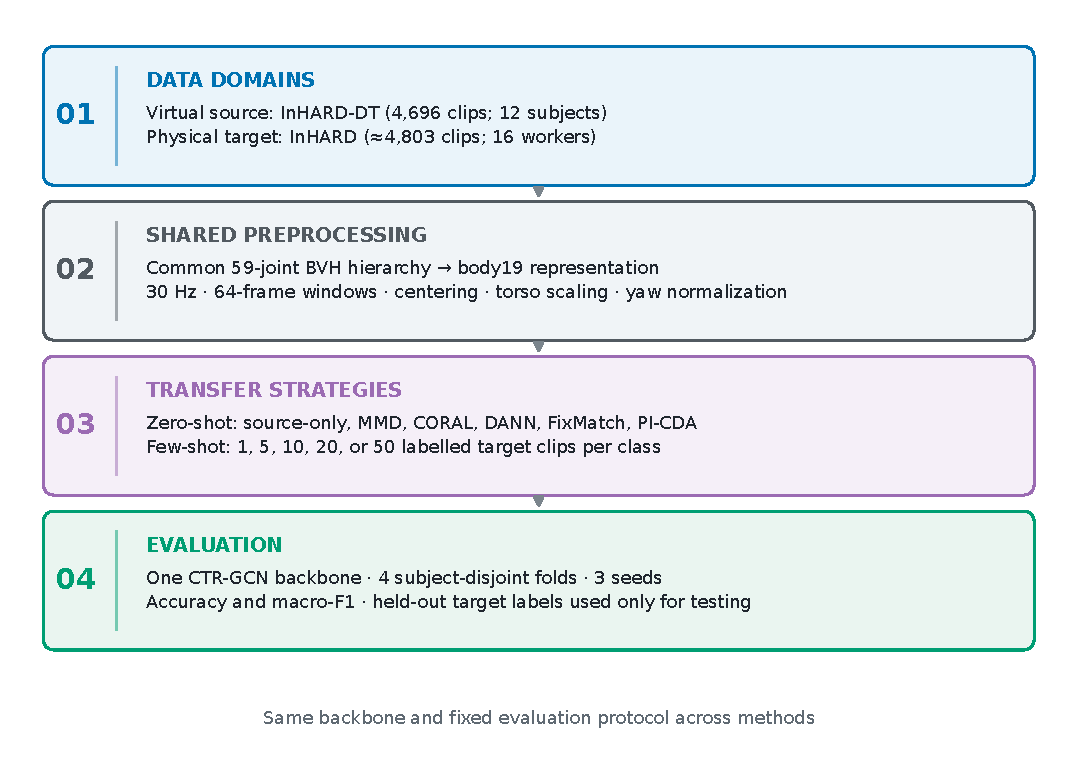
\includegraphics[width=0.9\textwidth]{../output_v2/benchmark_ctrgcn/figures/paper_ready/methodology.pdf}
  \caption{Four-stage workflow from paired datasets through harmonization and transfer to held-out evaluation.}
  \label{fig:methodology}
\end{figure}

\subsection{Problem Formulation}

Let $\mathcal{S}=\{(x_i^s,y_i^s)\}$ be labelled skeleton clips from the
digital-twin domain, and let $\mathcal{T}=\{x_j^t\}$ be unlabelled clips from
the physical workcell. For zero-shot transfer, we learn $f_\theta$ from
$\mathcal{S}$ and unlabelled $\mathcal{T}$, then evaluate it on held-out target
subjects. For few-shot adaptation, we also use a support set
$\mathcal{T}_k^\ell$ with $k$ labelled clips per class. Test subjects remain
disjoint from the source subjects and the target subjects used for adaptation.

\subsection{\acs{inharddt} and \acs{inhard}}

The \acs{inharddt} source domain contains 4,696 segmented clips from 12 subjects
across 26 sessions. Participants wore a Perception Neuron suit in a
virtual-reality replica of the workstation~\cite{dallel2023dataset}. The
\acs{inhard} physical target domain contains approximately 4,803 clips from 16
workers recorded with the same \ac{mocap} system family~\cite{dallel2020inhard}.
We exclude ``No action'' clips. Both datasets use the same 59-joint \ac{bvh}
hierarchy and 13 meso-level action classes. The experiment measures
transfer across physical context, worker population, execution style, and
workstation interaction, rather than transfer between sensors.
Figure~\ref{fig:dataset-collection} contains three original dataset images. The
upper-left image shows a participant as a virtual avatar in the InHARD-DT
workstation; the upper-right image shows four rendered views of that workstation
with its original panel labels. The lower image is the InHARD montage, showing
participants performing the assembly task alongside the corresponding skeleton
view. We reproduce all three images unchanged under the
\href{https://creativecommons.org/licenses/by/4.0/}{Creative Commons
  Attribution 4.0 International license}~\cite{dallel2023dataset,dallel2020inhard};
the InHARD-DT study describes the virtual capture setup~\cite{dallel2023digital}.

\begin{figure}[H]
  \centering
  \begin{minipage}[t]{0.485\linewidth}
    \vspace{0pt}\centering
    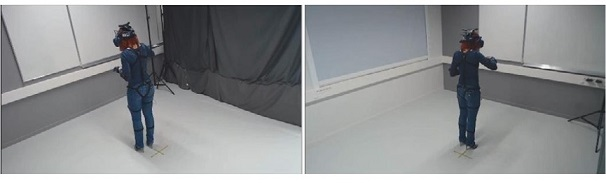
\includegraphics[width=\linewidth]{figures/dataset_collection/inhard_dt_vr_capture.jpg}
  \end{minipage}\hfill
  \begin{minipage}[t]{0.485\linewidth}
    \vspace{0pt}\centering
    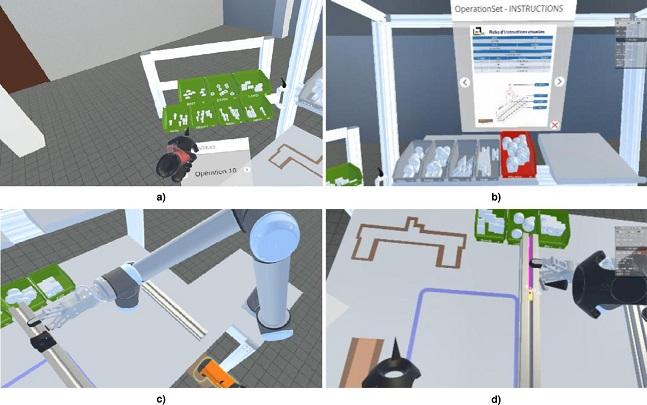
\includegraphics[width= \linewidth]{figures/dataset_collection/inhard_dt_workstation_views.jpg}
  \end{minipage}
  \par\smallskip
  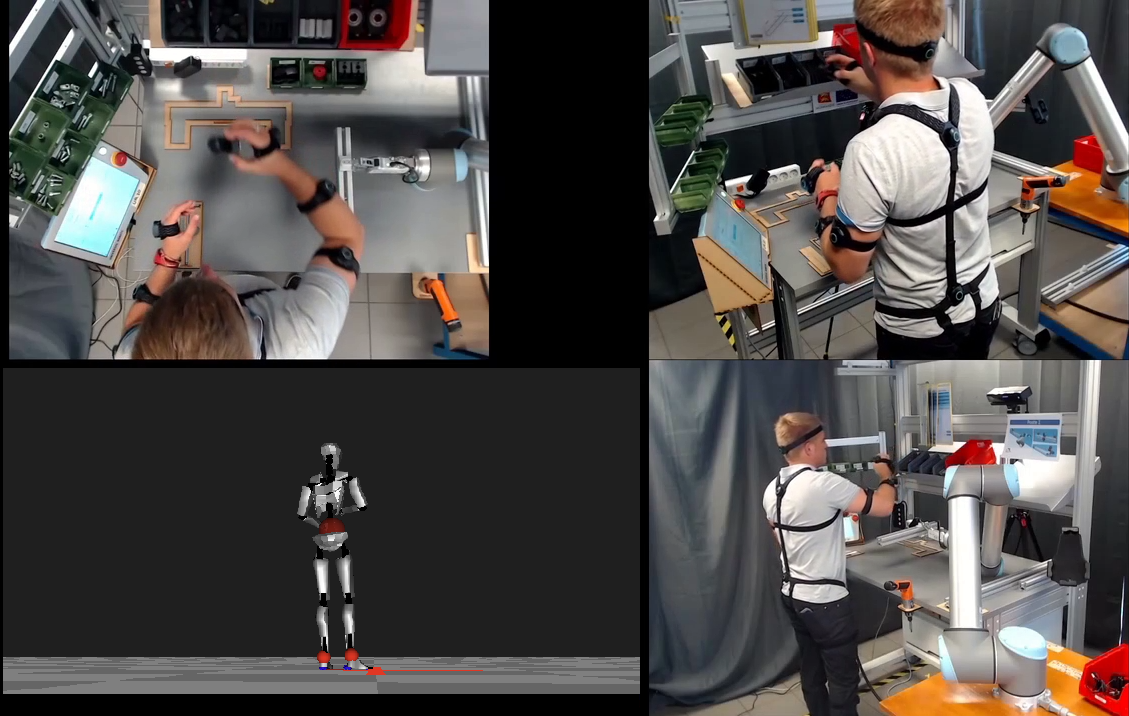
\includegraphics[width=0.5\linewidth]{figures/dataset_collection/inhard_physical_capture.png}
  \caption{Experimental setups for InHARD-DT and InHARD~\cite{dallel2023dataset,dallel2020inhard,dallel2023digital}.}
  \label{fig:dataset-collection}
\end{figure}

\subsection{Preprocessing}

We convert raw \ac{bvh} sequences into fixed-length clips at 30 Hz and retain a
19-joint body representation comprising the torso, limbs, wrists, and hand
landmarks used by the model. We canonicalise each clip by centring it on the
first frame, scaling by torso size, and normalising its initial facing yaw. This
reduces nuisance variation without using action labels or target-test
information. Skeleton-based recognition requires consistent representations
of body structure and temporal motion~\cite{liu2025skeletonreview,wang2025heterogeneous}.
Both domains use the same joint-coordinate representation and preprocessing
pipeline.

\subsection{Subject-disjoint folds}

We divide the 16 \acs{inhard} workers into four fixed test folds, each with four
workers. The remaining 12 workers in each fold form the target adaptation
pool. We use all \acs{inharddt} subjects for the source domain and exclude held-out
target workers from training; their labels are used only for final evaluation.
Unless noted otherwise, reported means and standard deviations cover four
folds and three seeds. For Wilcoxon signed-rank comparisons, we pair
seed-averaged per-subject macro-\acs{f1} values across the 16 target workers
using the saved fold assignments. We report uncorrected pairwise $p$-values as
exploratory results for this benchmark, not as equivalence tests across
datasets. Subject-independent validation helps assess generalisation to unseen
people, and recent human-activity-recognition comparisons examine how validation
choices affect reported performance~\cite{mekruksavanich2025validation}.

\subsection{Common recogniser}

All methods use the same \ac{ctrgcn} backbone, 64-frame windows, body19 input,
50 supervised epochs, batch size 64, and optimiser configuration recorded with
the benchmark outputs. This control prevents methods from benefiting from a
larger backbone or a different training budget. We train the source-only model
with source labels and evaluate it on the target test fold without target
labels. The \acs{dt} in-domain result provides a diagnostic upper bound for
cross-domain representation quality. The target oracle and source-plus-target
model show performance when target supervision is available. Recent
sensor-based activity-recognition work also uses graph-based domain adaptation,
which motivates testing transfer methods with a fixed
recogniser~\cite{yang2024domainhar}.

\subsection{Algorithm Selection}

We chose methods that test different explanations for transfer failure.
\ac{mmd} matches distributions with a kernel, \ac{coral} aligns second-order
statistics, and \ac{dann} learns adversarial domain invariance. \ac{fm} applies
confidence-filtered pseudo-label consistency between weak and strong target
views. Recent work analyses the generalisation of this semi-supervised
approach~\cite{li2024fixmatchanalysis}. Our \ac{picda} configuration tests a
project-specific physics-informed hypothesis by coupling feature alignment
with skeleton-topology consistency. Together, the methods cover marginal and
adversarial alignment, pseudo-labelling, and structure-aware regularisation.

The supervised controls answer three related questions. The source-only model
measures transfer without target supervision; the target oracle measures
performance when the target training pool is labelled; and source-plus-target
training tests whether source data remains useful once target labels are
available. The few-shot variants isolate the effect of the target-label budget
across seven initialisations: scratch, source-only, \ac{picda}, joint,
\ac{fm}, prototype, and prototype fine-tuning. All methods share the same
\ac{ctrgcn} backbone, data representation, fold assignment, training budget,
and final-model evaluation. Figure~\ref{fig:methodology} shows the method
selection and evaluation flow.

\subsection{Few-shot adaptation}

For each $k\in\{1,5,10,20,50\}$, the support set contains $k$ labelled target
clips per action class. We sample clips without replacement within each class
from the 12-worker adaptation pool. The sampling seed is $1000s+10f+k$, where
$s$ is the experiment seed and $f$ is the target fold. We save the selected clip
identifiers with each result. We compare seven initialisations: scratch,
source-only, \ac{picda}, joint source-target training, joint training with
\ac{fm}, joint training with a prototype objective, and joint prototype
fine-tuning. The final variant, \texttt{joint\_proto\_ft}, adapts the
digital-twin-trained representation using labelled target clips and a
prototype-aware objective. Recent work on cross-modal contrastive pre-training
for few-shot skeleton action recognition provides context for this
limited-label setting~\cite{lu2024crossmodalfewshot}. Support clips come only
from the 12-worker adaptation pool; the four-worker test fold remains untouched.

\subsection{Metrics and statistical protocol}

We report \ac{acc} and macro-\acs{f1}. Macro-\acs{f1} is the primary metric
because the 13 actions differ in difficulty and macro averaging weights each
class equally. Recent work compares macro, micro, and support-weighted
summaries in multi-label evaluation~\cite{lee2024f1metrics}. We compute means
and standard deviations over 12 fold-seed runs. Paired comparisons use saved
subject-level predictions and Wilcoxon signed-rank tests. Bootstrap intervals
are reported with their seed coverage and do not replace the complete 12-run
summaries. We do not use target test scores for early stopping or model and
method selection.

\section{Results}
\label{sec:results}

\subsection{Zero-shot transfer}

Table~\ref{tab:main} compares the in-domain reference, zero-shot source
transfer, five unsupervised adaptation methods, and two target-supervised
controls. Macro-\acs{f1} is the primary comparison because it gives equal
importance to each action class; the reported means and standard deviations
cover four subject-disjoint folds and three seeds.

\begin{table}[H]
  \centering
  \caption{\acs{inharddt} to \acs{inhard} transfer over four subject-disjoint folds and three seeds.}
  \label{tab:main}
  \small
  \begin{tabular}{lrr}
    \toprule
    Method             & \acs{acc} (\%)          & Macro-\acs{f1} (\%)     \\
    \midrule
    \acs{dt} in-domain & $75.47\pm3.54$          & $73.32\pm4.04$          \\
    Source-only        & $50.16\pm2.97$          & $\mathbf{40.59\pm2.93}$ \\
    \acs{dann}         & $46.71\pm3.89$          & $38.17\pm3.00$          \\
    \acs{coral}        & $48.17\pm4.00$          & $38.88\pm3.10$          \\
    \acs{mmd}          & $49.21\pm3.18$          & $39.66\pm3.00$          \\
    \acs{picda}        & $48.35\pm2.79$          & $39.34\pm2.50$          \\
    \acs{fm}           & $50.75\pm2.91$          & $40.54\pm2.93$          \\
    Target oracle      & $82.67\pm2.38$          & $75.22\pm4.04$          \\
    Source + target    & $\mathbf{83.95\pm1.98}$ & $\mathbf{75.89\pm3.20}$ \\
    \bottomrule
  \end{tabular}
\end{table}

This comparison evaluates recognition on unseen physical workers without
target labels and tests whether unsupervised adaptation reduces the transfer
gap. Each score covers four subject-disjoint folds, with four workers held out
per fold, and three random seeds (12 fold-seed runs). Source-only transfer
achieves
$40.59\pm2.93\%$ macro-\acs{f1}; \acs{dann}, \acs{coral}, \acs{mmd}, and
\acs{picda} achieve $38.17\pm3.00\%$, $38.88\pm3.10\%$, $39.66\pm3.00\%$,
and $39.34\pm2.50\%$, respectively, while \acs{fm} is effectively matched at
$40.54\pm2.93\%$. The \acs{picda} result is 1.25 points below source-only and
the paired difference is not significant ($p=0.105$). We find no reliable
zero-shot gain from the evaluated adaptation methods. The
target oracle reaches $75.22\pm4.04\%$ and joint source-target
training reaches $75.89\pm3.20\%$, compared with $73.32\pm4.04\%$ for the
digital-twin in-domain reference. The $34.63$-point gap between source-only
transfer and the target oracle points to generalisation across physical domains
as the main challenge. In the available paired comparison, the oracle and
source-plus-target results are statistically indistinguishable. Class-wise
results show the same uneven pattern: source-only performs well on \emph{Picking left}
($77.1\%$ \acs{f1}) but poorly on \emph{Consult sheets} ($12.5\%$),
\emph{Take component} ($18.8\%$), and \emph{Take subsystem} ($16.4\%$), for
which the oracle reaches $30.6\%$, $74.5\%$, and $60.8\%$, respectively.
Figure~\ref{fig:zeroshot} compares methods by macro-\acs{f1}; the dashed line
marks the source-only result. The earlier \acs{stgcn} study provides dataset
context~\cite{dallel2023digital}. Its results are not directly comparable with
this stricter \acs{ctrgcn} evaluation.

\begin{figure}[H]
  \centering
  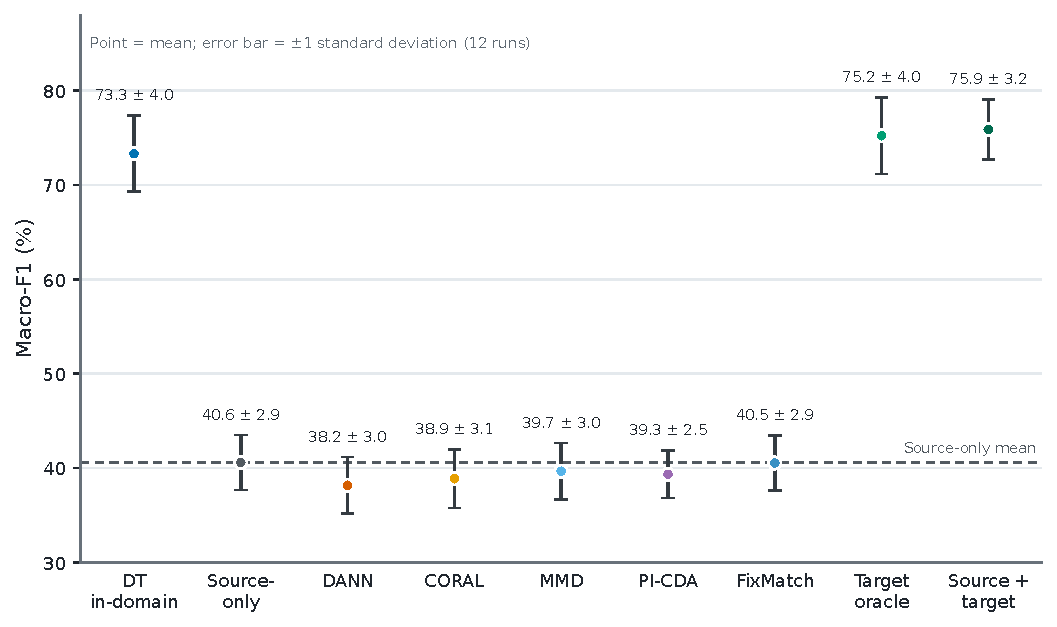
\includegraphics[width=.92\textwidth]{../output_v2/benchmark_ctrgcn/figures/paper_ready/zero_shot.pdf}
  \caption{Zero-shot virtual-to-physical transfer on the held-out physical domain.}
  \label{fig:zeroshot}
\end{figure}

\subsection{Effect of target-label budget}
\label{sec:label-budget}

Table~\ref{tab:fewshot} reports \acs{acc} and macro-\acs{f1} for joint
prototype fine-tuning at five physical-label budgets, alongside the target
oracle. Each value summarizes 12 fold-seed runs.

\begin{table}[H]
  \centering
  \caption{Few-shot target adaptation with joint prototype fine-tuning, all values use 12 runs.}
  \label{tab:fewshot}
  \small
  \begin{tabular}{rcc}
    \toprule
    Target clips per class & \acs{acc} (\%) & Macro-\acs{f1} (\%) \\
    \midrule
    1                      & $50.35\pm4.04$ & $41.22\pm4.38$      \\
    5                      & $57.91\pm3.44$ & $49.43\pm3.74$      \\
    10                     & $61.99\pm3.14$ & $54.52\pm3.35$      \\
    20                     & $67.17\pm3.16$ & $60.20\pm3.96$      \\
    50                     & $74.11\pm2.36$ & $66.27\pm3.46$      \\
    \midrule
    Target oracle          & $82.67\pm2.38$ & $75.22\pm4.04$      \\
    \bottomrule
  \end{tabular}
\end{table}

This experiment measures recognition when physical target clips are labelled
for adaptation. In each fold, we sample the support set from the 12-worker
adaptation pool and evaluate on the four held-out workers.
\texttt{joint\_proto\_ft} adapts the digital-twin-trained representation using
the labelled clips. Its performance improves
monotonically as the budget increases from 1 to 50 clips per class:
macro-\acs{f1} is
$41.22\pm4.38\%$, $49.43\pm3.74\%$, $54.52\pm3.35\%$, $60.20\pm3.96\%$,
and $66.27\pm3.46\%$, while \acs{acc} is $50.35\pm4.04\%$,
$57.91\pm3.44\%$, $61.99\pm3.14\%$, $67.17\pm3.16\%$, and
$74.11\pm2.36\%$, respectively. Compared with zero-shot source-only
macro-\acs{f1} ($40.59\%$), the gains are 0.63, 8.84, 13.93, 19.61, and
25.68 points. At 50 clips per class, the method reaches about 74\% of the
$34.63$-point gap between source-only transfer and the target oracle
($75.22\%$). Target labels improve performance over unsupervised
transfer. The curve does not establish whether digital-twin initialisation
outperforms other ways of using those labels; the initialization-strategy
comparison examines that question. Figure~\ref{fig:fewshot} plots both metrics
against the target-label budget, with means and standard deviations over 12
fold-seed runs.

\begin{figure}[H]
  \centering
  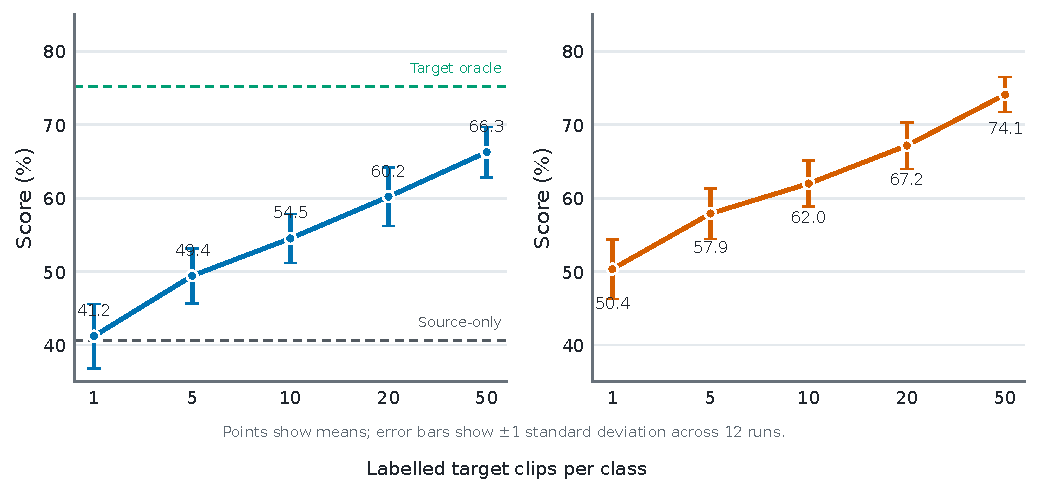
\includegraphics[width=.82\textwidth]{../output_v2/benchmark_ctrgcn/figures/paper_ready/few_shot.pdf}
  \caption{Accuracy and macro-\acs{f1} for joint prototype fine-tuning.}
  \label{fig:fewshot}
\end{figure}

\subsection{Comparison of initialization strategies}
\label{sec:initializations}

This comparison tests whether performance depends on how virtual-source and
physical-target data are combined, as well as on the number of target labels.
We use the same support-set sampling and held-out-worker evaluation across five
target-label budgets. Each plot compares seven strategies: training from
scratch, source-only, \acs{picda}, joint source-target training, joint training
with \acs{fm}, joint training with a prototype objective, and joint prototype
fine-tuning. Horizontal position shows mean macro-\acs{f1}; whiskers show one
standard deviation over 12 fold-seed runs. Green identifies the numerical
leader for a budget and does not indicate statistical significance.

With one labelled clip per class, joint training with a prototype objective
has the highest mean macro-\acs{f1} ($43.17\pm4.08\%$), 13.89 points above
few-shot source-only. The nearest joint configuration reaches $42.50\%$; the
difference in means alone does not establish a significant advantage.
Figure~\ref{fig:init-k1} shows the one-shot comparison.

\begin{figure}[H]
  \centering
  \IfFileExists{../output_v2/benchmark_ctrgcn/figures/paper_ready/initializations_k1.pdf}
  {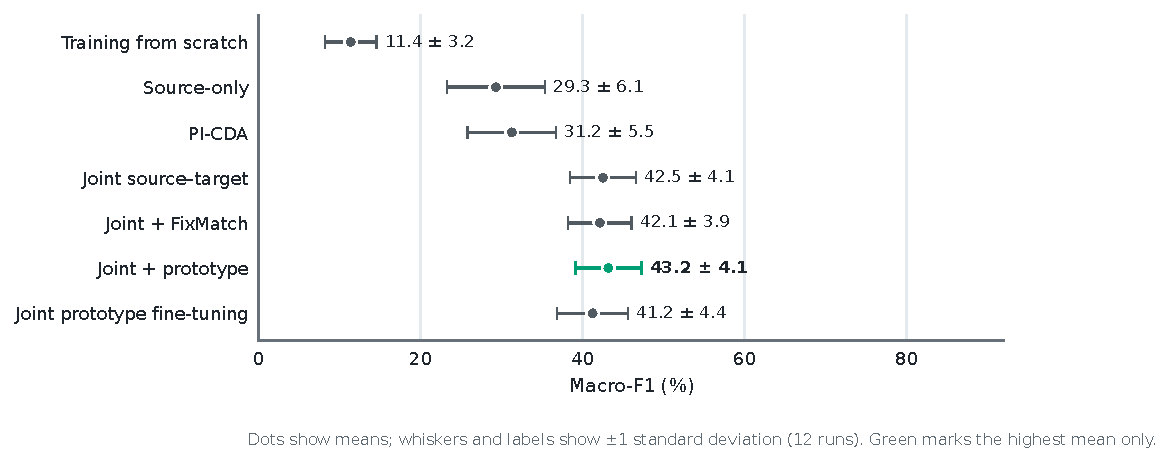
\includegraphics[width=.98\textwidth]{../output_v2/benchmark_ctrgcn/figures/paper_ready/initializations_k1.pdf}}
  {\fbox{\parbox[c][2.5cm][c]{.9\linewidth}{\centering
        Initialization plot not generated. Run \texttt{create\_result\_figures.py}.}}}
  \caption{Initialization strategies with 1 labelled target clip per class.}
  \label{fig:init-k1}
\end{figure}

With 5 labelled clips per class, joint prototype fine-tuning reaches
$49.43\pm3.74\%$ macro-\acs{f1}, 3.79 points above few-shot source-only.
Figure~\ref{fig:init-k5} compares the strategy means and their run-to-run
variability at this budget.

\begin{figure}[H]
  \centering
  \IfFileExists{../output_v2/benchmark_ctrgcn/figures/paper_ready/initializations_k5.pdf}
  {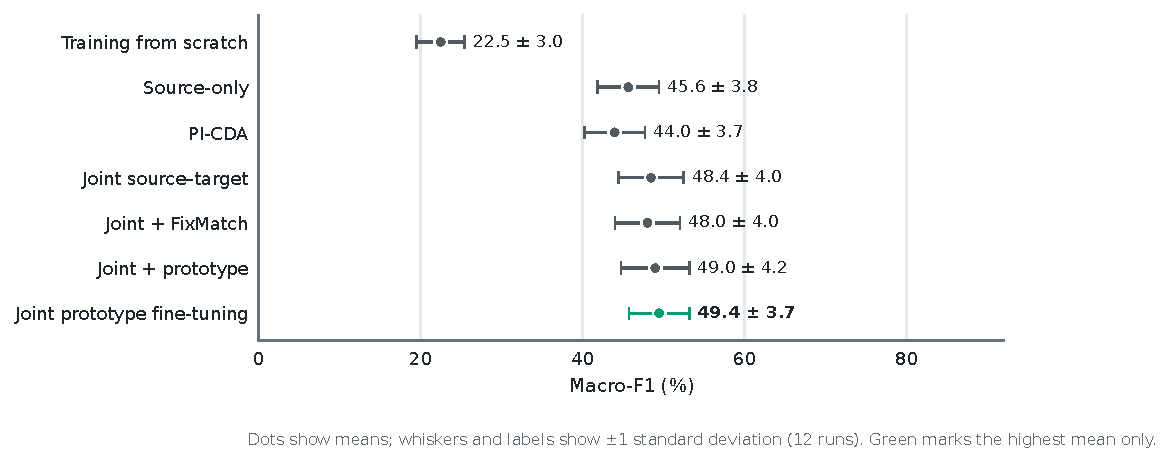
\includegraphics[width=.98\textwidth]{../output_v2/benchmark_ctrgcn/figures/paper_ready/initializations_k5.pdf}}
  {\fbox{\parbox[c][2.5cm][c]{.9\linewidth}{\centering
        Initialization plot not generated. Run \texttt{create\_result\_figures.py}.}}}
  \caption{Initialization strategies with 5 labelled target clips per class.}
  \label{fig:init-k5}
\end{figure}

With 10 labelled clips per class, joint prototype fine-tuning reaches
$54.52\pm3.35\%$ macro-\acs{f1}, compared with $53.10\%$ for few-shot
source-only, a difference of 1.42 points. Figure~\ref{fig:init-k10} shows the
seven strategies at this budget. The difference between the leading means is
descriptive and does not establish statistical significance.

\begin{figure}[H]
  \centering
  \IfFileExists{../output_v2/benchmark_ctrgcn/figures/paper_ready/initializations_k10.pdf}
  {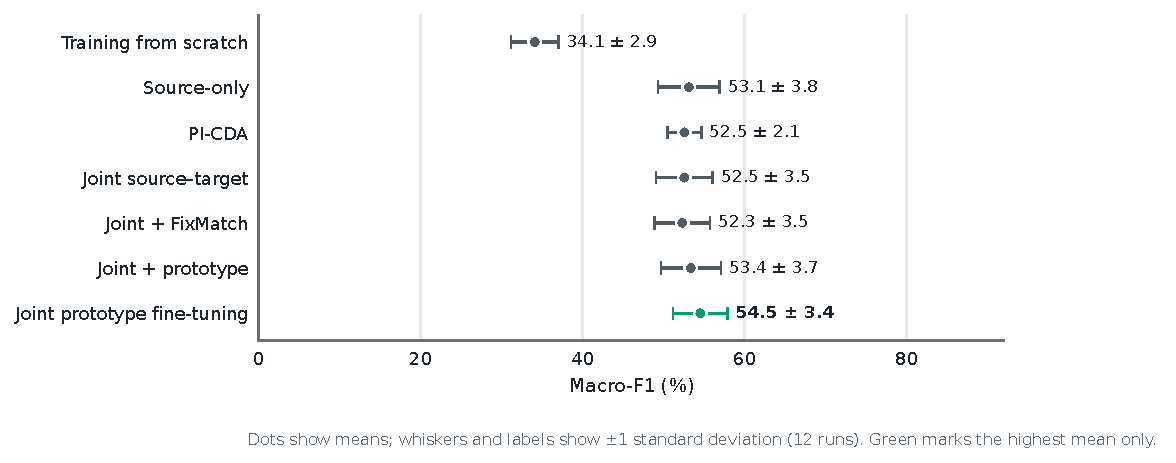
\includegraphics[width=.98\textwidth]{../output_v2/benchmark_ctrgcn/figures/paper_ready/initializations_k10.pdf}}
  {\fbox{\parbox[c][2.5cm][c]{.9\linewidth}{\centering
        Initialization plot not generated. Run \texttt{create\_result\_figures.py}.}}}
  \caption{Initialization strategies with 10 labelled target clips per class.}
  \label{fig:init-k10}
\end{figure}

With 20 labelled clips per class, joint prototype fine-tuning reaches mean
macro-\acs{f1} of $60.20\pm3.96\%$, 1.09 points above few-shot source-only
($59.11\%$). Figure~\ref{fig:init-k20} shows this budget separately. The
small difference between the leading means should be read in light of the
run-to-run variability.

\begin{figure}[H]
  \centering
  \IfFileExists{../output_v2/benchmark_ctrgcn/figures/paper_ready/initializations_k20.pdf}
  {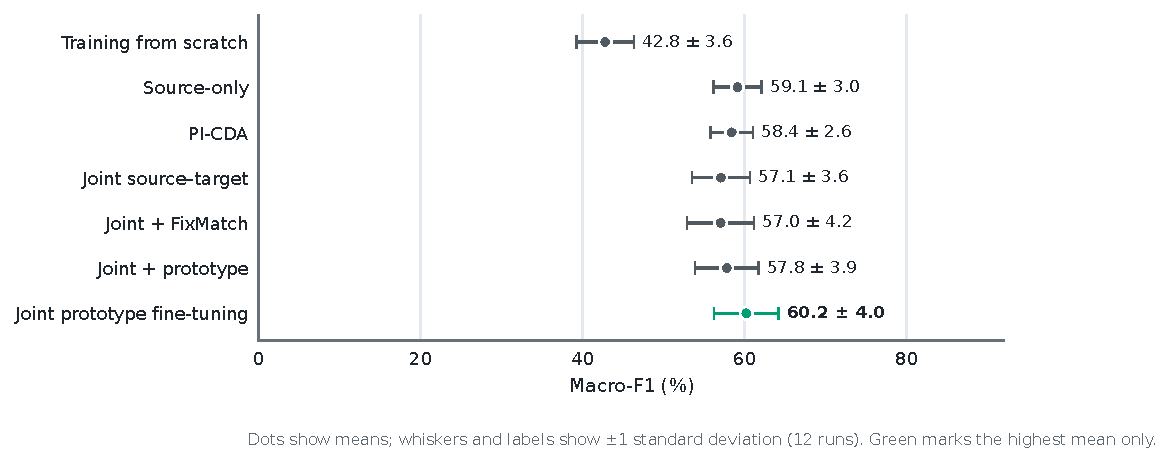
\includegraphics[width=.98\textwidth]{../output_v2/benchmark_ctrgcn/figures/paper_ready/initializations_k20.pdf}}
  {\fbox{\parbox[c][2.5cm][c]{.9\linewidth}{\centering
        Initialization plot not generated. Run \texttt{create\_result\_figures.py}.}}}
  \caption{Initialization strategies with 20 labelled target clips per class.}
  \label{fig:init-k20}
\end{figure}

At 50 labelled clips per class, joint prototype fine-tuning reaches
$66.27\pm3.46\%$ macro-\acs{f1}, 1.28 points above few-shot source-only
($64.99\%$). Figure~\ref{fig:init-k50} shows this budget separately. The
leading strategy varies by budget, and its mean advantage over source-only is
modest from 5 clips per class onward.

\begin{figure}[H]
  \centering
  \IfFileExists{../output_v2/benchmark_ctrgcn/figures/paper_ready/initializations_k50.pdf}
  {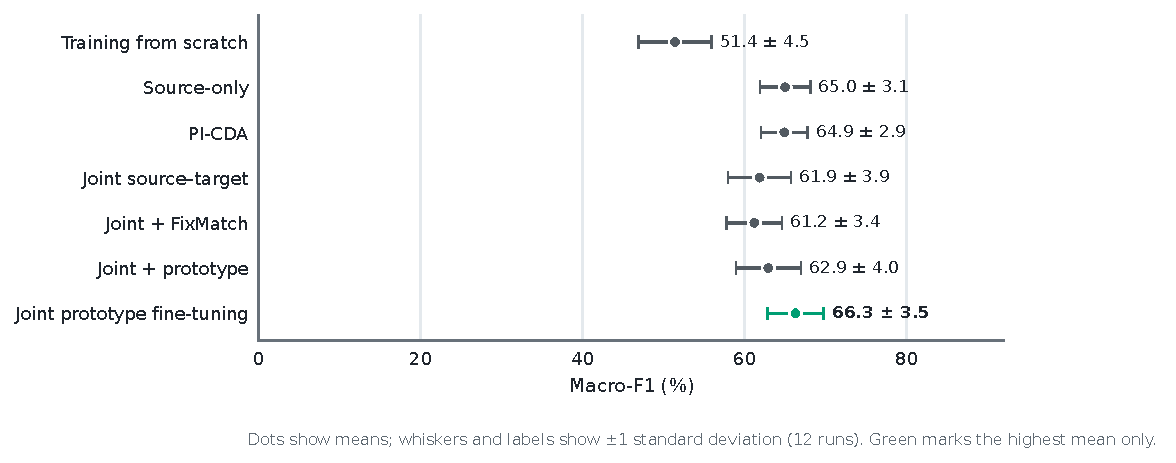
\includegraphics[width=.98\textwidth]{../output_v2/benchmark_ctrgcn/figures/paper_ready/initializations_k50.pdf}}
  {\fbox{\parbox[c][2.5cm][c]{.9\linewidth}{\centering
        Initialization plot not generated. Run \texttt{create\_result\_figures.py}.}}}
  \caption{Initialization strategies with 50 labelled target clips per class.}
  \label{fig:init-k50}
\end{figure}

The experiments cover zero-shot transfer to held-out physical workers, the
effect of adding physical labels, and the performance of alternative
initialization and adaptation strategies. The evaluated unsupervised methods
do not reliably improve on source-only transfer, so these results do not show
that the digital twin alone closes the virtual-to-physical domain gap.
Performance rises with the target-label budget. Prototype-based adaptation
performs competitively with one labelled clip per class, but its numerical
advantage over few-shot source-only is modest at larger budgets and does not
establish statistical significance. These results characterize zero-shot
transfer and label-efficient adaptation under a controlled, subject-disjoint
protocol. They do not establish a general solution or a replacement for
physical data. The findings apply to the tested InHARD-DT-to-InHARD pair,
shared \acs{ctrgcn} backbone, and evaluation protocol; testing on additional
datasets and workcells is needed to assess their broader relevance.

\section{Discussion}
\label{sec:discussion}

\subsection{What the digital twin does and does not provide}

The in-domain \acs{dt} result does not predict physical deployment performance:
macro-\acs{f1} falls from 73.32\% in-domain to 40.59\% under source-only
transfer. The shared \acs{bvh} hierarchy and canonical skeleton reduce
representational nuisance, but the domain gap remains. \acs{picda} does not
improve zero-shot transfer in this benchmark, which marks a limit of the
evaluated configuration.

Target supervision improves few-shot performance, but the results do not show
that digital-twin pretraining accounts for the full gain. Training from
scratch is weakest, while the prototype-based strategy has the highest mean at
each budget. Its margin over few-shot source-only is largest with one clip per
class and modest from 5 to 50 clips. Digital-twin data may provide a
useful starting point when labels are scarce, although additional physical
labels remain important and no tested initialization consistently produces a
large advantage over the other few-shot strategies.

\subsection{Implications for deployment}

For a new workcell, one possible procedure is to pretrain on the digital twin,
collect a small, class-balanced calibration set from the target worker
population, and adapt without using held-out workers' labels. The required
budget depends on risk tolerance and class costs. In this benchmark, 20 to 50
clips per class outperform one-shot calibration by a substantial margin. The
target oracle remains an upper bound, not an operational requirement.

\subsection{Threats to validity}

The benchmark has four limitations. First, it uses one source-target pair and
one primary backbone. Generalisation to other robots, sensors, and action
taxonomies remains untested; our findings characterize this transfer setting
and do not establish how all digital twins or adaptation methods behave.
Second, the few-shot support-set sampling and class distribution are specific
to this protocol. Third, we evaluate recognition on held-out workers, not
closed-loop robot assistance, so improved \acs{f1} does not establish safety.
Fourth, the statistical comparison file contains bootstrap intervals with
limited seed coverage. We base the primary claims on complete 12-run
summaries and paired fold-subject analyses. Further evaluation should include
multiple workcells and risk-sensitive measures.

% \section{Reproducibility and Data Availability}
% \label{sec:reproducibility}

% The preprocessing code, model implementations, benchmark runner, saved
% predictions, summary tables, and analysis notebook are maintained in the
% project's \texttt{04\_Cross\_Modal\_Digital\_Twin} directory. The benchmark
% configuration records the body19 representation, 64-frame window, canonical
% centering, torso scaling, initial-yaw normalisation, four folds, and three
% seeds. Results are resumable at the individual fold-seed JSON level. The
% public \acs{inharddt} and \acs{inhard} source records are identified in
% Section~\ref{sec:methodology}; users should follow their access and citation
% requirements. The source and target datasets are available through Zenodo
% records 7644247 and 4003541, respectively, subject to the access conditions
% specified by their maintainers~\cite{dallel2023dataset,dallel2020inhard}.

\section{Conclusion}
\label{sec:conclusion}

Collecting labelled recordings from every worker and workcell is costly, which
makes digital-twin data attractive for industrial action recognition. However,
virtual recordings may not represent how workers move and interact with
equipment in a physical cell. We examined this transfer problem using InHARD-DT
as the source and InHARD as the target. With a shared CTR-GCN backbone, we
compared source-only transfer and unsupervised adaptation under four
subject-disjoint folds and three random seeds, then evaluated few-shot
adaptation with target labels while keeping test workers held out.

The results show that the tested unsupervised methods did not reliably improve
zero-shot performance: source-only transfer reached 40.59\% macro-\acs{f1},
compared with 39.34\% for \acs{picda}. With 50 labelled target clips per class,
joint prototype fine-tuning reached 66.27\%, below the 75.22\% target oracle.
The gains as the label budget increased show that digital-twin pretraining can
provide a starting point for adaptation, while physical labels remain important.
Further work should test this finding across more workcells, worker groups, and
sensing conditions, and evaluate whether recognition gains support calibrated,
risk-sensitive robot assistance.
\newpage
\bibliographystyle{elsarticle-harv}
\bibliography{references}
\end{document}
